\documentclass[crop,tikz]{standalone}% 'crop' is the default for v1.0, before it was 'preview'
\usetikzlibrary{positioning,shapes.geometric}
\usepackage{tikz}

\begin{document}
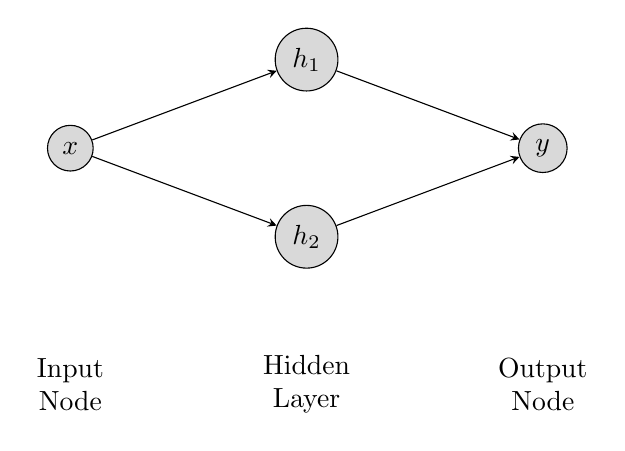
\begin{tikzpicture}[x=1.5cm, y=1.5cm, >=stealth]

% Input node
\node[circle, draw=black, fill=gray!30] (I) at (0,0) {$x$};

% Hidden layer
\node[circle, draw=black, fill=gray!30] (H1) at (2,0.75) {$h_1$};
\node[circle, draw=black, fill=gray!30] (H2) at (2,-0.75) {$h_2$};

% Output node
\node[circle, draw=black, fill=gray!30] (O) at (4,0) {$y$};

% Connections
\draw[->] (I) -- (H1);
\draw[->] (I) -- (H2);
\draw[->] (H1) -- (O);
\draw[->] (H2) -- (O);

% Labels
\node[align=center] at (0,-2) {Input\\Node};
\node[align=center] at (2,-2) {Hidden\\Layer};
\node[align=center] at (4,-2) {Output\\Node};

\end{tikzpicture}
\end{document}

